\documentclass{article}
\usepackage[utf8]{inputenc}
\usepackage{multicol}

\usepackage{listings}
\usepackage{geometry}
\usepackage{color}
\usepackage{pdflscape}
\usepackage{float}
\usepackage{amsmath}
\usepackage{hyperref}
\setlength{\belowcaptionskip}{-10pt}
\setlength{\abovecaptionskip}{-30pt}
\floatstyle{boxed} 
\restylefloat{figure}
\usepackage{graphicx}
\definecolor{codegreen}{rgb}{0,0.6,0}
\definecolor{codegray}{rgb}{0.5,0.5,0.5}
\definecolor{codepurple}{rgb}{0.58,0,0.82}
\definecolor{backcolour}{rgb}{0.95,0.95,0.92}

\lstdefinestyle{mystyle}{
	backgroundcolor=\color{backcolour},   
	commentstyle=\color{codegreen},
	keywordstyle=\color{blue},
	numberstyle=\tiny\color{codegray},
	stringstyle=\color{codepurple},
	basicstyle=\footnotesize,
	breakatwhitespace=false,         
	breaklines=true,                 
	captionpos=b,                    
	keepspaces=true,                 
	numbers=left,                    
	numbersep=5pt,                  
	showspaces=false,                
	showstringspaces=false,
	showtabs=false,                  
	tabsize=2
}
\renewcommand{\theenumi}{\Alph{enumi}}
\lstset{style=mystyle}
\title{Data Mining\\
		Home work 02\\ Descriptive Statistics}
\author{\textbf{Student:}Aqeel Labash\\ \textbf{Teacher:} Jaak Vilo}
\date{18 February 2016}
\geometry{
	a4paper,
	total={170mm,257mm},
	left=1mm,
	right=1mm,
	top=5mm,
	bottom=5mm,
}
\usepackage{enumitem}
\begin{document}
	\maketitle

\begin{multicols*}{2}
{	\centering	\section*{First Question}}
	\begin{enumerate}[label=\Alph*)]
		\item \textbf{Columns Names:}Gender , Length, Diameter,Height, Weight, Rings.
		\item \textbf{Number of Rows:}1000.
		\item \textbf{Print First 3 Lines ,and Rings Values:} The code for this task is 
		\begin{lstlisting}[language=R]
rm(list = ls())
setwd('/home/aqeel/Study/DM/HW02')
mydata = read.csv('abalone.csv')
colnames(mydata)
length(mydata)
nrow(mydata)
mydata[(1:3),]
		\end{lstlisting}
		The result was this table :
		
		\begin{tabular}{|c|c|c|c|c|c|c|}
			\hline
			&Gender&Length&Diameter&Height&Weight&Rings\\
			\hline
			1&F&0.505&0.385&0.135&0.6185&12\\
			\hline
			2&F&0.650&0.475&0.165&1.3875&9\\
			\hline
			3&I&0.520&0.380&0.135&0.5395&8\\
			\hline
		\end{tabular}
			The Rings values :12,9,8
		\item \textbf{Last two data rows \& there Weight}:
		The code for this question:
		\begin{lstlisting}[language=R]
#print last two rows
mydata[c(nrow(mydata),nrow(mydata)-1),]
#print last two rows weight
mydata[c(nrow(mydata),nrow(mydata)-1),]$Weight
		\end{lstlisting}
		And here is the result table :\\
		\resizebox{\columnwidth}{!}{%
		\begin{tabular}{|c|c|c|c|c|c|c|}
			\hline
			&Gender&Length&Diameter&Height&Weight&Rings\\
			\hline
			1000&M&0.515&0.395&0.135&1.0070&8\\
			\hline
			999&I&0.525&0.400&0.130&0.6455&8\\
			\hline
		\end{tabular} %
	}
		The weight for the last two : 1.0070 and 0.6455
		\item \textbf{Diameter value of row 755}:0.385 achieved by this code:
		\begin{lstlisting}[language=R]
#print diameter of row 755
mydata[755,]$Diameter
		\end{lstlisting}
		\item \textbf{The number of missing values in height column:} 4, the code for this request:
		\begin{lstlisting}[language=R]
		#number of rows that don't have height value
		length(mydata[is.na(mydata)])
		\end{lstlisting}
		\item \textbf{The mean of Height value excluding NA's:} The value is :0.1398092 achieved by this code:
		\begin{lstlisting}[language=R]
		#the mean for height column (two ways)
		mean(mydata[complete.cases(mydata),]$Height)
		mean(mydata[!is.na(mydata$Height),]$Height)
		\end{lstlisting}
		
		\item \textbf{Extract Subset and it's Diameter mean:} The code for this task is below : 
		\begin{lstlisting}[language=R]
#Extract subset with Gender M and weight less than 0.75
newsubset = subset(mydata,mydata$Gender=="M" & mydata$Weight<0.75)
		\end{lstlisting}
		There was 119 object satisfy the previous condition.The mean value for the diameter :0.3426471
		\item \textbf{Most frequent rings value:} 9 Discovered through this code:
		\begin{lstlisting}[language=R]
			#Most frequent rings value
			table(mydata$Rings)
		\end{lstlisting}
			\item \textbf{Minimum length when Rings equal 18:}0.465.Following the code I used for this request
			\begin{lstlisting}[language=R]
			#minimum length when rings equal to 18
			min(subset(mydata,Rings==18)$Length)
			\end{lstlisting}
	\end{enumerate}

{\centering\section*{Second Question}}


	\begin{flushleft}
\begin{enumerate}

 \item \textbf{The data is about:} The data about Abalone or sea ears which belong to the family of Haliotidae (one genus).\cite{1} The data describe the animal sex,length,diameter,height,weight.
 \item \textbf{Discrete and continuous features:}The \textbf{discrete features} are gender and rings.The \textbf{continuous features} are length,weight,diameter,height.
 \item \textbf{Number of rows:}1000 (if you calculate the header as a row it's 1001 :) )
 \item \textbf{More info about features:}\\
 To calculate those information for (gender) I'll replace the values (M,F,I) to (1,2,3), \textbf{Note:} I feel that discrete features shouldn't be measured as continuous feature but I'll do it since it's requested:)).
 \begin{tabular}{|c|c|c|c|c|c|}
\hline
feature&mean&median&min&max&SD\\
\hline
Length&0.52276&0.5450&0.075&0.815&0.12006\\
\hline
Diameter&0.405955&0.42&0.055&0.650&0.09883\\
\hline
Height&0.1398092&0.1425&0.0&1.130&0.04942\\
\hline
Weight&0.8255405&0.801&0.002&2.555&0.49037\\
\hline
Rings&11.318&9.0&1.0&1500.0&47.22769665\\
\hline
Gender&2.016&2&1&3&0.78636020\\
\hline
 \end{tabular}
The code for the previous table  :
\begin{lstlisting}[language=R]
gender<-mydata$Gender
gender<- as.numeric(factor(mydata$Gender,c('F','M','I'),c(1:3)))
#Extract All Required Information
values <-rbind(
#Length
c(mean(mydata$Length),median(mydata$Length),min(mydata$Length),max(mydata$Length),sd(mydata$Length)),
#Diameter
c(mean(mydata$Diameter),median(mydata$Diameter),min(mydata$Diameter),max(mydata$Diameter),sd(mydata$Diameter)),
#Height
c(mean(mydata$Height,na.rm = TRUE),median(mydata$Height,na.rm = TRUE),min(mydata$Height,na.rm = TRUE),max(mydata$Height,na.rm = TRUE),sd(mydata$Height,na.rm = TRUE)),
#Weight
c(mean(mydata$Weight),median(mydata$Weight),min(mydata$Weight),max(mydata$Weight),sd(mydata$Weight)),
#Rings
c(mean(mydata$Rings),median(mydata$Rings),min(mydata$Rings),max(mydata$Rings),sd(mydata$Rings)),
#Gender
c(mean(Gender),median(Gender),min(Gender),max(Gender),sd(Gender)))
values
\end{lstlisting}

\end{enumerate}
\end{flushleft}

The distribution for the features is as following : 
\begin{figure}[H]
	\label{fig:ggplotLength}
	\begin{center}
	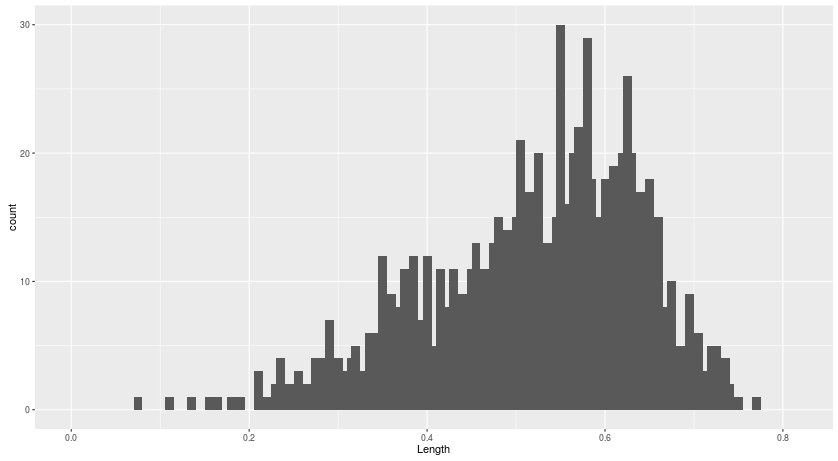
\includegraphics[scale=0.3]{ggplotLength.png}
	\end{center}
	\caption{Abalone Length Distribution }
\end{figure}
As shown in figure 1 we can see that Length values are very small. The distribution is clearly skewed to the left.\cite{2}
\begin{figure}[H]
	\begin{center}
		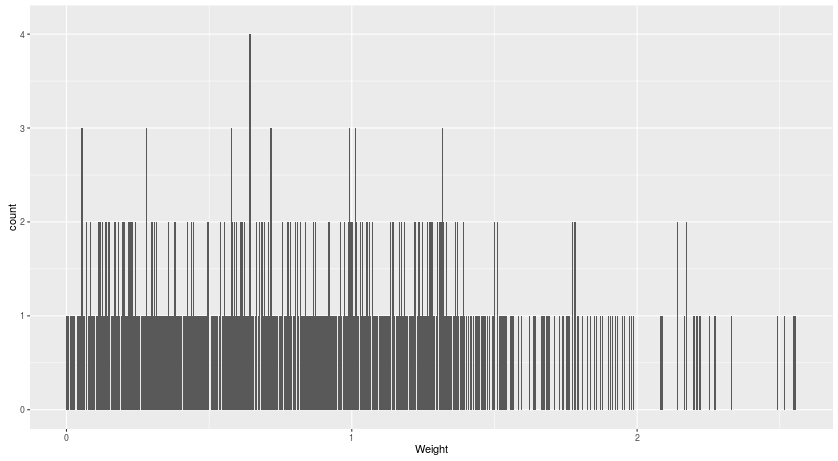
\includegraphics[scale=0.3]{ggplotweight.png}
	\end{center}
	\caption{Abalone weight distribution}
\end{figure}
The weight values are well distributed but most of it to the left side.
\begin{figure}[H]
\begin{center}
	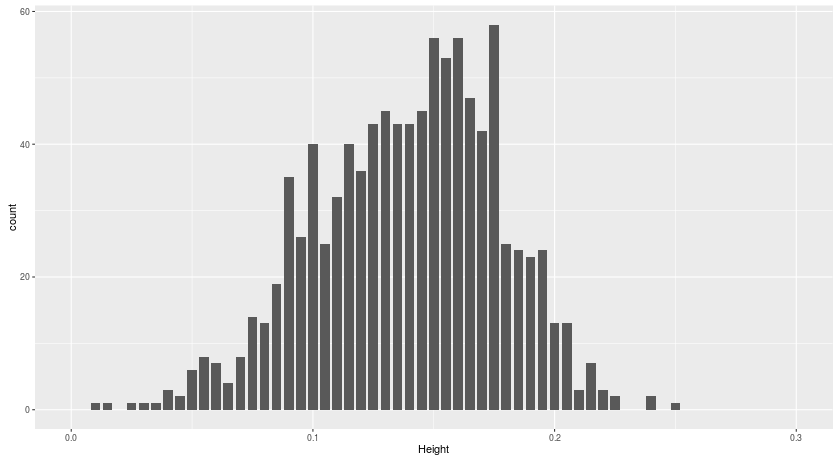
\includegraphics[scale=0.3]{ggplotHeight.png}
\end{center}
\caption{Abalone Height Distribution}
\end{figure}
Abalone height somehow not very skewed (slightly skewed to left).Abalone height value is very small with some exception excluded from the previous figure for better view.
\begin{figure}[H]
	\begin{center}
		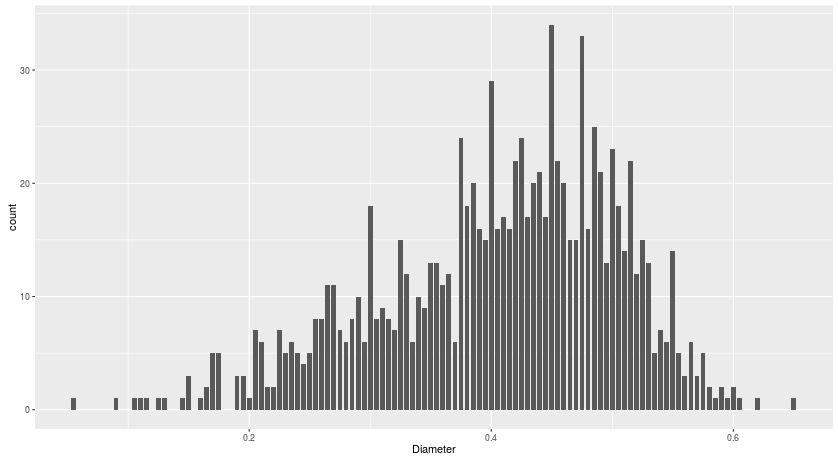
\includegraphics[scale=0.3]{ggplotdiameter.png}
	\end{center}
	\caption{Abalone diameter distribution}
\end{figure}
Most of the values are small.The values skewed to the left.
\begin{figure}[H]
	\begin{center}
		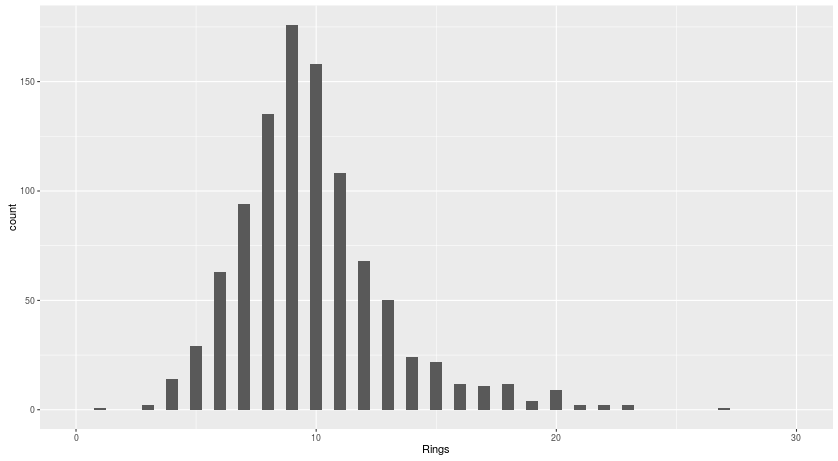
\includegraphics[scale=0.3]{ggplotRings.png}
	\end{center}
	\caption{Abalone rings distribution}
\end{figure}
Most values between 1 and 30. The distribution almost perfect (it's skewed a little bit to the right)
\begin{figure}[H]
	\begin{center}
		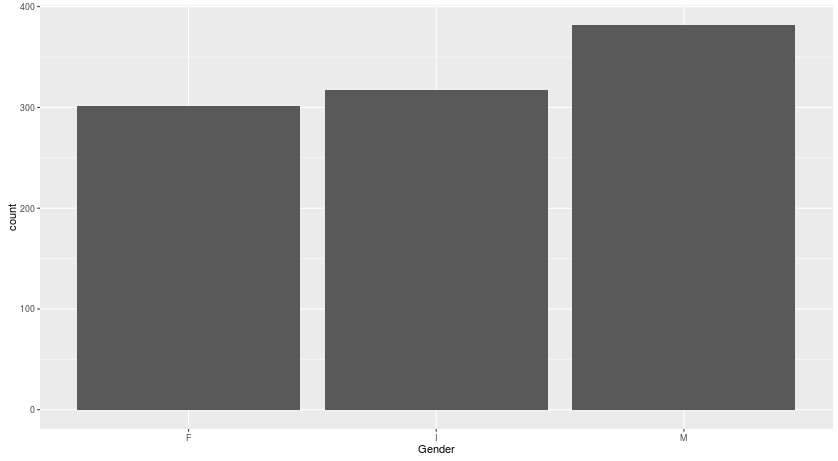
\includegraphics[scale=0.3]{ggplotGender.png}
	\end{center}
	\caption{Abalone gender distribution}
	Nothing much to say about figure 6
\end{figure}

figures from 1 to 5 were generated by the following code:
\begin{lstlisting}[language=R]
#Rings
ggplot(mydata, aes(x=Rings))+stat_count(width=0.5)+xlim(0,30)
#Length
ggplot(mydata, aes(x=Length))+geom_bar(width=0.01)+xlim(0,0.815)
#Diameter
ggplot(mydata,aes(x=Diameter))+geom_bar(width = 0.004)
#Weight
ggplot(mydata,aes(x=Weight))+geom_bar(width = 0.004)+ylim(0,4.1)
#Height
ggplot(mydata,aes(x=Height))+geom_bar(width = 0.004)+xlim(0,0.3)
#Gender
ggplot(mydata,aes(x=Gender))+stat_count(width = 0.9)
\end{lstlisting}
\end{multicols*}
\begin{landscape}
{\centering\section*{Third Question}}
\begin{figure}[H]
	\begin{center}
		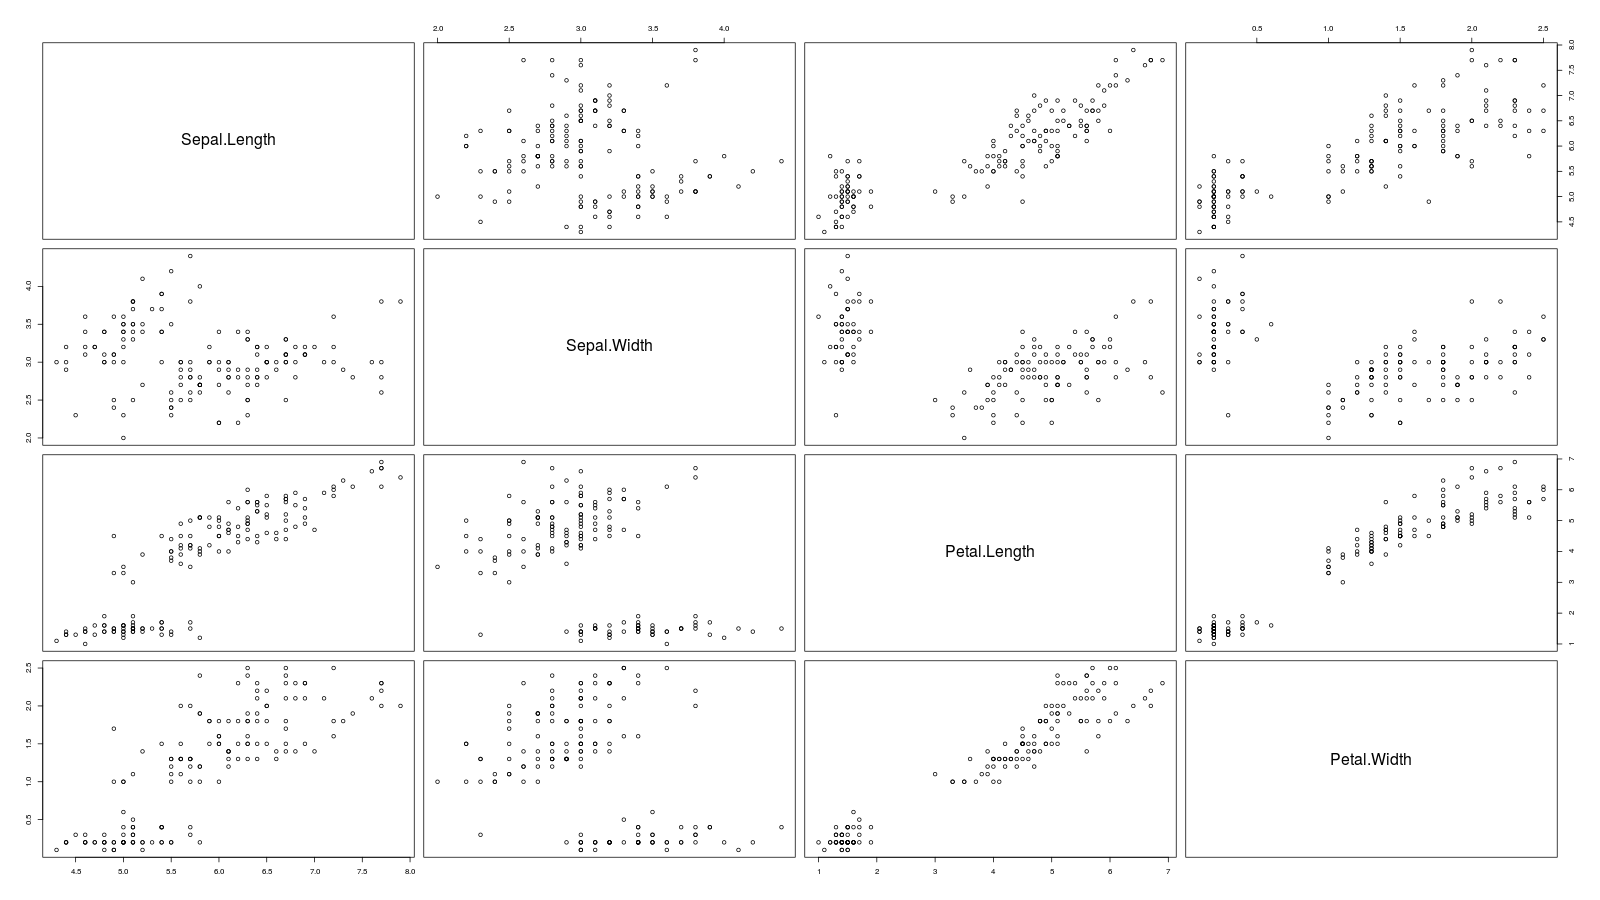
\includegraphics[scale=0.5]{scatterplotall.png}
	\end{center}
\end{figure}
\end{landscape}

\begin{multicols*}{2}
{\centering \section*{Continuing  Third Question}}
The previous plot was generated by this code:
\begin{lstlisting}[language=R]
#Save plot with high resultion
png("scatterplotall.png",width = 1600,height = 900)
#draw plot
plot(mydata[,2:6])
#write plot
dev.off()
\end{lstlisting}
To calculate the correlation between all variables I used this code: 
\begin{lstlisting}[language=R]
#Print correlation
cor(mydata[complete.cases(mydata),][,2:6])
\end{lstlisting}
The result was the following table.\\
	\resizebox{\columnwidth}{!}{%
\begin{tabular}{|c|c|c|c|c|c|c|}
\hline
		&Length&Diameter&Height&Weight&Rings\\
		\hline
		Length&1.00000000&0.98747396&0.68725941&0.92071393&0.04407577\\
		\hline
		Diameter&0.98747396&1.00000000&0.69249343&0.92348680&0.03787742\\
		\hline
		Height&0.68725941&0.69249343&1.00000000&0.67393746&0.03112661\\
		\hline
		Weight&0.92071393&0.92348680&0.67393746&1.00000000&0.03385043\\
		\hline
		Rings&0.04407577&0.03787742&0.03112661&0.03385043&1.00000000\\
		\hline
		%
\end{tabular}
		}
From the table we can see that Length is the most correlated feature with Rings.
\begin{figure}[H]
	\begin{center}
		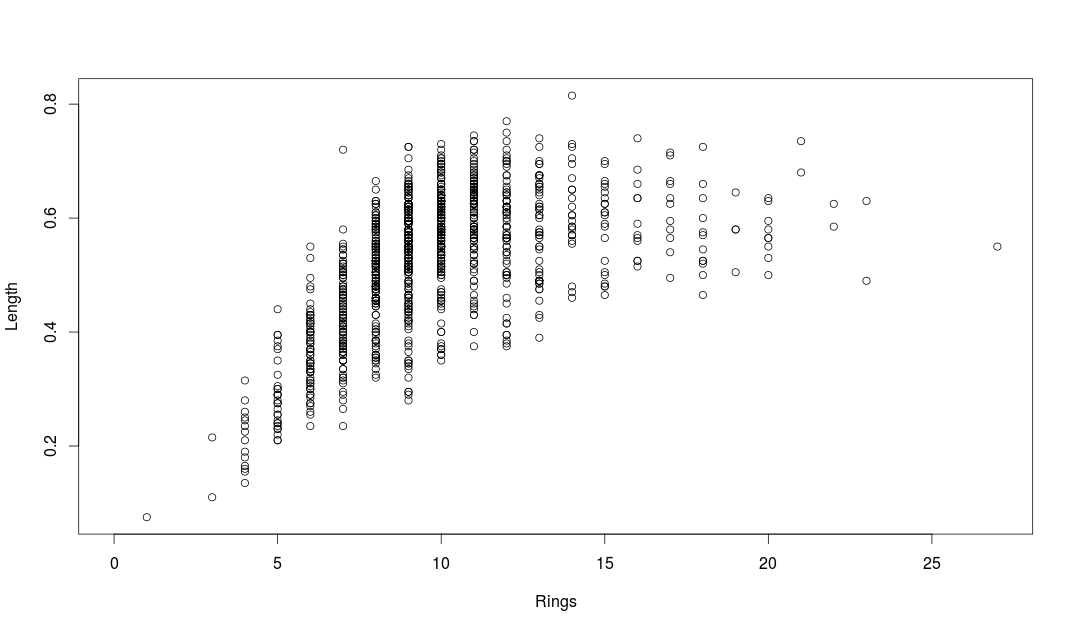
\includegraphics[scale=0.28]{scatterplotLengthRings.png}
	\end{center}
	\caption{Scatterplot showing correlation between length and rings}
\end{figure}
\textbf{Note:}in figure 7 I specified X domain to (0,27) to make the figure viewable. Here is the code:
\begin{lstlisting}[language=R]
#scatterplot
plot(mydata$Rings,mydata$Length,xlim = c(0,27),xlab = "Rings",ylab = "Length")
\end{lstlisting}
To get the most correlated two features we can check correlation table we created earlier. Diameter and length are the most correlated features and here is the scatter plot for them:
\begin{figure}[H]
	\begin{center}
		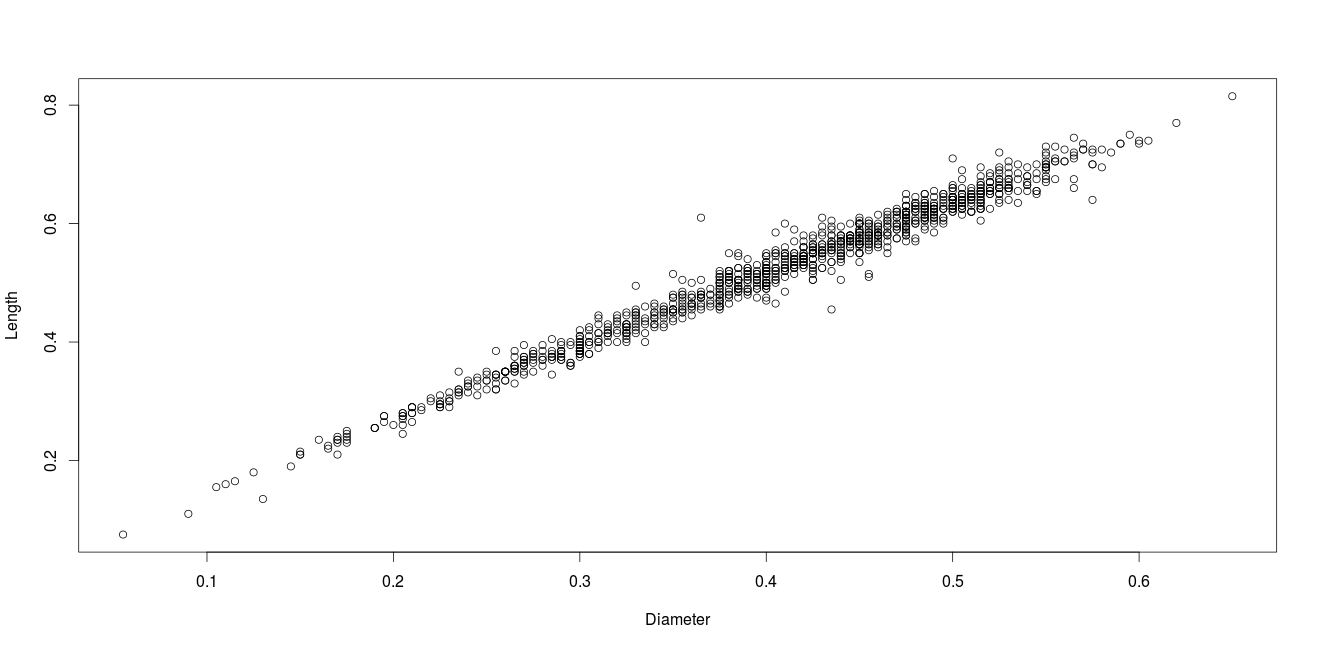
\includegraphics[scale=0.22]{scatterplotDiameterLength.png}
	\end{center}
	\caption{Scatter plot for diameter and length}
\end{figure}
What I notice is it's almost for each unique value for diameter there is only few correspondent value on length.Which mean they are linked to each other. Mathematically make sense since it's a relation between length and diameter.
{\centering \section*{Fourth Question}}
The IQR (Inter-Quartile Ranges) for values shown in this table:\\
\begin{tabular}{|c|c|c|c|c|}
	\hline
Length&Diameter&Height&Weight&Rings\\
\hline
0.165000&0.135000&0.050000&0.707375&3.000000\\
\hline
\end{tabular}\\
The values extracted by this code :
\begin{lstlisting}[language=R]
IQRFunction<-function(x)
{
return (quantile(x,0.75) - quantile(x,0.25) )
}
height<- mydata[complete.cases(mydata),]
IQRALL= c(IQRFunction(mydata$Length),IQRFunction(mydata$Diameter),IQRFunction(height$Height),IQRFunction(mydata$Weight),IQRFunction(mydata$Rings))
names(IQRALL)<- names(mydata)[2:6]
IQRALL
\end{lstlisting}
The total number of values (over,under) the quartiles in the following table:\\
\begin{tabular}{|c|c|c|c|c|c|}
	\hline
	&Length&Diameter&Height&Weight&Rings\\
	\hline
	Over&0&0&2&9&56\\
	\hline
	Under&8&7&6&0&3\\
	\hline
\end{tabular}
\\The previous values where achieved by the following code : 
\begin{lstlisting}[language=R]
#Calculate Over outlier
outliercounttop<-function(x,iqr)
{
return (length(which(x>(quantile(x,0.75)+1.5*iqr))))
}
#Calculate Under outlier
outliercountfloor<-function(x,iqr)
{
return (length(which(x<(quantile(x,0.25)-1.5*iqr))))
}
names(IQRALL)
matr <-rbind(c(outliercounttop(mydata$Length,IQRALL[1]),outliercounttop(mydata$Diameter,IQRALL[2]),
outliercounttop(height$Height,IQRALL[3]),outliercounttop(mydata$Weight,IQRALL[4]),
outliercounttop(mydata$Rings,IQRALL[5])),
c(outliercountfloor(mydata$Length,IQRALL[1]),outliercountfloor(mydata$Diameter,IQRALL[2]),
outliercountfloor(height$Height,IQRALL[3]),outliercountfloor(mydata$Weight,IQRALL[4]),
outliercountfloor(mydata$Rings,IQRALL[5])))
colnames(matr)<-names(mydata)[2:6]
rownames(matr)<-(c("Over","Under"))
matr
\end{lstlisting}
For multidimensional outliers I believe they do exist in the data but I think if we removed them depending on one side that will remove them.\\
In the other hand an observation might be over or under outliers for one variable but not for the another.

{\centering \section*{Fifth Question}}
I do believe we should remove them and I think so because :
\begin{enumerate}
	\item They are away from the mean or median.
	\item Usually they are minority and will act as noise more than rule.
\end{enumerate}
The ones that should be deleted : height,length I will exclude rings, because I think the top 56 element in rings are correlated with other features.But maybe we can remove the highest one (1500 ring).\\
Firstly, I cleaned the data by this code:
The result in the following table:\\
\begin{tabular}{|c|c|c|c|c|c|c|}
	\hline
feature&mean&median&min&max&SD\\
\hline
Length&0.5258215&0.5450&0.21&0.815&0.11577628\\
\hline
Diameter&0.4084229&0.4225&0.15&0.650&0.09566371\\
\hline
Height&0.1396907&0.1450&0.00&0.250&0.03706943\\
\hline
Weight&0.8323337&0.8085&0.04&2.555&0.48757002\\
\hline
Rings&9.8894523&9.0000&3.00&27.000&3.09985267\\
\hline
Gender&2.0081136&2.0000&1.00&3.000&0.78432298\\
\hline
\end{tabular}
And here is the same previous value for better comparison:\\
 \begin{tabular}{|c|c|c|c|c|c|}
 	\hline
 	feature&mean&median&min&max&SD\\
 	\hline
 	Length&0.52276&0.5450&0.075&0.815&0.12006\\
 	\hline
 	Diameter&0.405955&0.42&0.055&0.650&0.09883\\
 	\hline
 	Height&0.1398092&0.1425&0.0&1.130&0.04942\\
 	\hline
 	Weight&0.8255405&0.801&0.002&2.555&0.49037\\
 	\hline
 	Rings&11.318&9.0&1.0&1500.0&47.22769665\\
 	\hline
 	Gender&2.016&2&1&3&0.78636020\\
 	\hline
 \end{tabular}
 The first thing to notice is the min,max values which is clearly because we removed the highest \&lowest values.Secondly we see that standard deviation is better now specially Rings.SD for rings shifted from 47.22~ to 3.09 which make more sense.The code to clear the data:
\begin{lstlisting}[language=R]
#Clean Length
mydata<-mydata[(mydata$Length<(quantile(mydata$Length,0.75)+1.5*IQRALL[1])) & 
(mydata$Length>(quantile(mydata$Length,0.25)-1.5*IQRALL[1])),]
#clean Height
mydata<-mydata[!is.na(mydata$Height),]
mydata<-mydata[(mydata$Height<(quantile(mydata$Height,0.75)+1.5*IQRALL[1])) & 
(mydata$Height>(quantile(mydata$Height,0.25)-1.5*IQRALL[1])),]
#clean Rings
mydata<-mydata[mydata$Rings<1500,]
nrow(mydata)
\end{lstlisting}
\textbf{Note:}Used the same code to get the values.
{\centering \section*{Sixth Question}}
For this question I used lm function in R to get the answer
\begin{lstlisting}[language=R]
#######################################
#           Sixth Question            #
#######################################
#USED MACHINE LEARNING EXERCISE SESSION CODE TO HELP WITH THIS TASK
rm(list=ls())
setwd("/home/aqeel/Study/DM/HW02/")
mydata = read.csv('abalone.csv',header = TRUE)
# Lets observe the data
plot(mydata[,c(3,5)])

# Lets observe the linear model
linear.model = lm(Weight ~ Diameter,mydata)
# Lets extract coeficiens of the linear model
variables <- coef(linear.model)
plot(mydata[,c(3,5)])
abline(a = variables[1],b = variables[2],col="red",lwd=5)
\end{lstlisting}
In figure 9 we can see the line that have the minimum MSE.
\begin{figure}[H]
\begin{center}
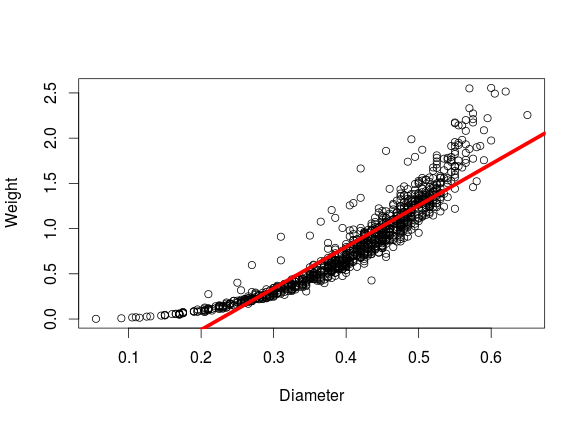
\includegraphics[scale=0.5]{plotprediction.png}
\end{center}
\caption{Weights and diameter with line used to minimize MSE}
\end{figure}
\textbf{Please Note:} attached with the report 3 *.R files contain all the R code for this home work.\\

\begin{thebibliography}{9}
	\bibitem{1} 
	\href{https://en.wikipedia.org/wiki/Abalone}{Wikipedia - Abalone}
	\bibitem{2}
	\href{http://study.com/academy/lesson/skewed-distribution-examples-definition-quiz.html}{Skewed Distribution}
\end{thebibliography}
\end{multicols*}

\end{document}